% !TEX TS-program = XeLaTeX
% !TeX program = xelatex

\documentclass[11pt]{article}
\usepackage[a4paper,left=15mm,right=15mm,top=20mm,bottom=20mm]{geometry}
\usepackage{authblk}
\usepackage{minted}
\usepackage{booktabs}
\usepackage[table]{xcolor}
\usepackage{pgfplots}
\usepackage{hyperref}
\usepackage{xcolor}
\usepackage{float}
\pgfplotsset{compat=1.18}

\setminted{
	linenos,                % show line numbers
	frame=single,           % frame around code
	breaklines,             % wrap long lines
	autogobble,             % remove common leading indentation
	fontsize=\small,
	bgcolor=gray!5,         % light gray background
}

\hypersetup{
    colorlinks=true,
    linkcolor=black,
    filecolor=blue,
    urlcolor=blue,
}

\title{\textbf{Connected Components Detection in Large Scale Graphs}}

\author{\textbf{Gerasimou Dimitrios} and \textbf{Stavrianidis Giannis}}

\affil{Department of Electrical and Computer Engineering\\
Aristotle University of Thessaloniki\\
050: Parallel and Distributed Systems\vspace{6pt}\\
Thessaloniki, Greece\\
November, 2025}

\date{}

\begin{document}

\maketitle
\thispagestyle{empty}

\begin{abstract}
This project efficiently identifies connected components in large undirected graphs containing
millions of nodes and edges. We implemented two algorithmic approaches—label propagation and
union-find—using three parallel programming paradigms (OpenMP, POSIX Threads, and OpenCilk)
to exploit multicore parallelism. Results demonstrate speedups ranging from 1.89× to 5.39× on 8
threads across seven diverse datasets, with OpenCilk achieving the best performance for label
propagation. We employ compressed sparse column (CSC) format for memory-efficient graph
representation and optimize performance through four key techniques: work chunking, partial
pointer jumping, bitmap-based component counting, and thread-local variables.
\end{abstract}

\section{Introduction}

A connected component is a maximal subgraph in which every vertex is reachable from any other
vertex. Identifying these components is fundamental in graph analysis, with applications in social
network analysis, web graph clustering, and biological network studies. The challenge lies in
processing graphs with hundreds of millions of nodes and edges within realistic memory and runtime
constraints. This work focuses on parallel implementations that leverage modern multicore
architectures to accelerate computation while maintaining correctness.

\section{Graph Representation}

We represent graphs using a custom Compressed Sparse Column (CSC) binary matrix structure that stores
only the adjacency structure, discarding numerical values:

\begin{minted}{c}
typedef struct {
        size_t   nrows, ncols;    /* Matrix dimensions */
        size_t   nnz;             /* Number of edges */
        uint32_t *row_idx;        /* Row indices (length = nnz) */
        uint32_t *col_ptr;        /* Column pointers (length = ncols + 1) */
} CSCBinaryMatrix;
\end{minted}

\section{Algorithmic Approaches}
\subsection{Label Propagation (Variant 0)}
The label propagation algorithm iteratively updates each vertex's label to the minimum label among
its neighbors. Vertices in the same connected component eventually converge to the same label. This
approach is naturally parallel-friendly since vertex updates within an iteration can be performed
independently. We parallelize the neighbor inspection loop using work chunking—dividing graph
columns into contiguous blocks and assigning each block to a thread. Convergence is detected when
no vertex changes its label in an iteration. To optimize performance, we incorporate partial pointer
jumping, where vertices can quickly adopt distant labels by following chains, significantly reducing
iteration counts.

\subsection{Union-Find (Variant 1)}
The union-find approach uses a disjoint-set data structure with path halving to efficiently merge
vertex sets as edges are processed. Each vertex initially belongs to its own set, and sets are merged
when edges are encountered. We parallelize by dividing edges among threads for local merging, then
combining parent pointers using thread-local variables and OpenMP reductions or Cilk reducers to
avoid race conditions. While union-find is typically the fastest sequential algorithm, its work is less
naturally divisible, resulting in smaller relative speedups compared to label propagation despite better
absolute performance.

\section{Parallelization Strategies}
We implemented three parallel programming paradigms:
\begin{itemize}
	\item \textbf{OpenMP:} Compiler-directive-based parallelism using: \texttt{\#pragma omp parallel for} with \\
	\texttt{schedule(static, chunk\_size)} for load-balanced work distribution

	\item \textbf{POSIX Threads:} Manual thread management with explicit work division, where each thread
	processes a contiguous block of columns

	\item \textbf{OpenCilk:} Work-stealing scheduler using \texttt{cilk\_for} for dynamic load balancing, particularly
	effective for irregular workloads
\end{itemize}

Each paradigm offers distinct trade-offs. OpenMP provides ease of implementation with good
performance. PThreads offer fine-grained control but requires manual synchronization. OpenCilk
excels at load balancing through work stealing, making it particularly effective for irregular graphs.

\section{Performance Optimizations}
We implemented four key optimizations: \textbf{(1) Work chunking} groups 
columns into chunks to reduce scheduling overhead and improve cache locality. 
\textbf{(2) Pointer jumping} enables vertices to adopt distant labels by 
following parent chains, accelerating convergence. \textbf{(3) Bitmap-based 
counting} replaces quicksort with constant-time membership testing for 
component identification. \textbf{(4) Thread-local variables} with reductions 
eliminate atomic operations and false sharing, improving scalability.

\section{Experimental Results}
\textbf{System Configuration:} Intel Core i7-11800H (8 cores), 16GB RAM, 16GB Swap on Arch Linux.
\begin{table}[htbp]
	\centering
	\rowcolors{2}{gray!10}{white}  % Start from row 2, alternate colors
	% \small
	\begin{tabular}{rllllll}
		\toprule
		\textbf{Index} & \textbf{Dataset} & \textbf{Nodes} & \textbf{Edges} & \textbf{Result} & \textbf{V0 Best (×)} & \textbf{V1 Best (×)}\\
		\midrule
		1 & dictionary28      & 52,652      & 178,076     & 17,903    & 3.90 (OpenMP)   & 2.59 (OpenMP)   \\
		2 & hollywood-2009    & 1,139,905   & 113,891,327 & 44,508    & 4.73 (OpenCilk) & 2.60 (OpenMP)   \\
		3 & kmer\_V1r         & 214,005,017 & 465,410,904 & 9         & 3.14 (OpenCilk) & 2.73 (OpenCilk) \\
		4 & kmer\_A2a         & 170,728,175 & 360,585,172 & 5353      & 2.40 (OpenMP)   & 2.75 (OpenCilk) \\
		5 & com-LiveJournal   & 3,997,962   & 69,362,378  & 1         & 5.11 (OpenCilk) & 3.82 (OpenMP)   \\
		6 & mawi              & 226,196,185 & 480,047,894 & 3,971,144 & 1.89 (OpenMP)   & 2.11 (OpenCilk) \\
		7 & com-Orkut         & 3,072,441   & 234,370,166 & 1         & 5.39 (OpenCilk) & 5.10 (OpenMP)   \\
		\bottomrule
	\end{tabular}
	\caption{Dataset characteristics and best speedup achieved by each algorithm 
	variant on 8 threads.\\ V0 = Label Propagation, V1 = Union-Find. Result column 
	shows number of connected components found.}
\end{table}

Figures \ref{fig:V0-speedup} and \ref{fig:V1-speedup} compare implementation speedups across datasets for variants 
0 and 1 respectively, while Figure \ref{fig:thread-speedup} examines strong scaling behavior.

\begin{figure}[H]
	\centering
	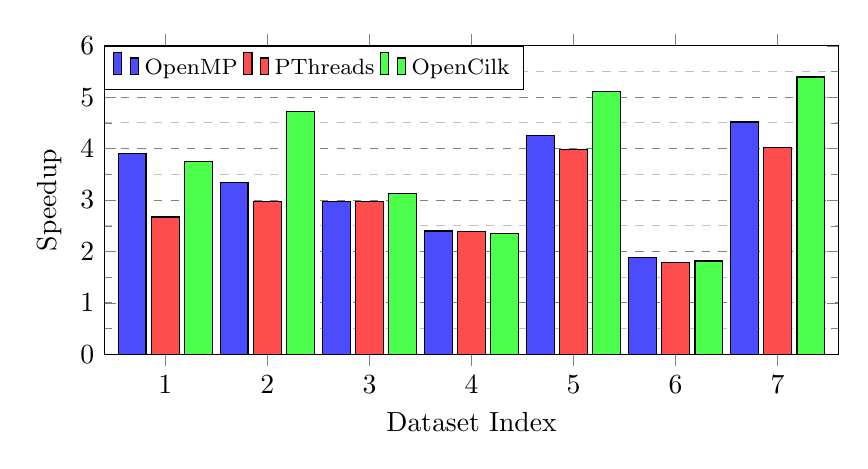
\begin{tikzpicture}
		\begin{axis}[
			ybar,
			width=0.9\textwidth,
			height=5.5cm,
			bar width=10pt,
			ylabel={Speedup},
			xlabel={Dataset Index},
			symbolic x coords={dictionary28, hollywood-2009, kmer\_V1r, kmer\_A2a, LiveJournal, mawi\_201512020330, Orkut},
			xtick=data,
			legend style={at={(0,1)}, anchor=north west, legend columns=3, font=\footnotesize},
			ymin=0,
			ymax=6,
			ymajorgrids=true,
			yminorgrids=true,
			minor y tick num=1,
			grid style={dashed, black!50},
			ytick={0,1,2,3,4,5,6},
			minor grid style={dashed, gray!50},
			xticklabels={1,2,3,4,5,6,7},
		]

		% OpenMP
		\addplot[fill=blue!70] coordinates {
			(dictionary28,3.9007) (hollywood-2009,3.3359) (kmer\_V1r,2.9731) (kmer\_A2a,2.3989) 
			(LiveJournal,4.2568) (mawi\_201512020330,1.8899) (Orkut,4.5182)
		};

		% PThreads
		\addplot[fill=red!70] coordinates {
			(dictionary28,2.67) (hollywood-2009,2.9641) (kmer\_V1r,2.9794) (kmer\_A2a,2.3933) 
			(LiveJournal,3.9917) (mawi\_201512020330,1.7882) (Orkut,4.0246)
		};

		% OpenCilk
		\addplot[fill=green!70] coordinates {
			(dictionary28,3.7516) (hollywood-2009,4.7259) (kmer\_V1r,3.1351) (kmer\_A2a,2.3563) 
			(LiveJournal,5.1131) (mawi\_201512020330,1.8141) (Orkut,5.3933)
		};

		\legend{OpenMP, PThreads, OpenCilk}

		\end{axis}
	\end{tikzpicture} \vspace{-12pt}
	\caption{Speedup comparison across seven datasets for label propagation (Variant 0) 
	using OpenMP, PThreads, and OpenCilk on 8 threads.}
	\label{fig:V0-speedup}
\end{figure}

\begin{figure}[H]
	\centering
	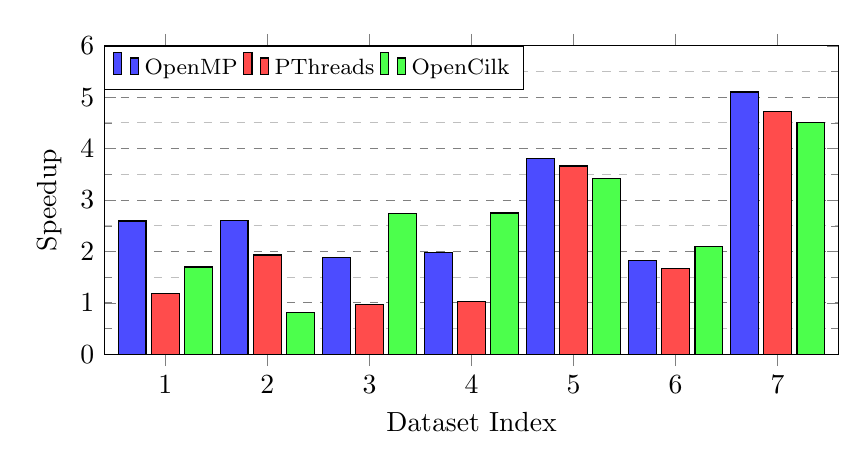
\begin{tikzpicture}
		\begin{axis}[
			ybar,
			width=0.9\textwidth,
			height=5.5cm,
			bar width=10pt,
			ylabel={Speedup},
			xlabel={Dataset Index},
			symbolic x coords={dictionary28, hollywood-2009, kmer\_V1r, kmer\_A2a, LiveJournal, mawi\_201512020330, Orkut},
			xtick=data,
			legend style={at={(0,1)}, anchor=north west, legend columns=3, font=\footnotesize},
			ymin=0,
			ymax=6,
			ymajorgrids=true,
			yminorgrids=true,
			minor y tick num=1,
			grid style={dashed, black!50},
			ytick={0,1,2,3,4,5,6},
			minor grid style={dashed, gray!50},
			xticklabels={1,2,3,4,5,6,7},
		]

		% OpenMP
		\addplot[fill=blue!70] coordinates {
			(dictionary28,2.5939) (hollywood-2009,2.6048) (kmer\_V1r,1.8754) (kmer\_A2a,1.9850) 
			(LiveJournal,3.8155) (mawi\_201512020330,1.8239) (Orkut,5.1026)
		};

		% PThreads
		\addplot[fill=red!70] coordinates {
			(dictionary28,1.1905) (hollywood-2009,1.9314) (kmer\_V1r,0.9654) (kmer\_A2a,1.0257) 
			(LiveJournal,3.6631) (mawi\_201512020330,1.6687) (Orkut,4.7214)
		};

		% OpenCilk
		\addplot[fill=green!70] coordinates {
			(dictionary28,1.6984) (hollywood-2009,0.8075) (kmer\_V1r,2.7332) (kmer\_A2a,2.7494) 
			(LiveJournal,3.4112) (mawi\_201512020330,2.1055) (Orkut,4.5130)
		};

		\legend{OpenMP, PThreads, OpenCilk}

		\end{axis}
	\end{tikzpicture} \vspace{-12pt}
	\caption{Speedup comparison across seven datasets for union-find (Variant 1) 
	using OpenMP, PThreads, and OpenCilk on 8 threads.}
	\label{fig:V1-speedup}
\end{figure}

\begin{figure}[H]
	\centering
	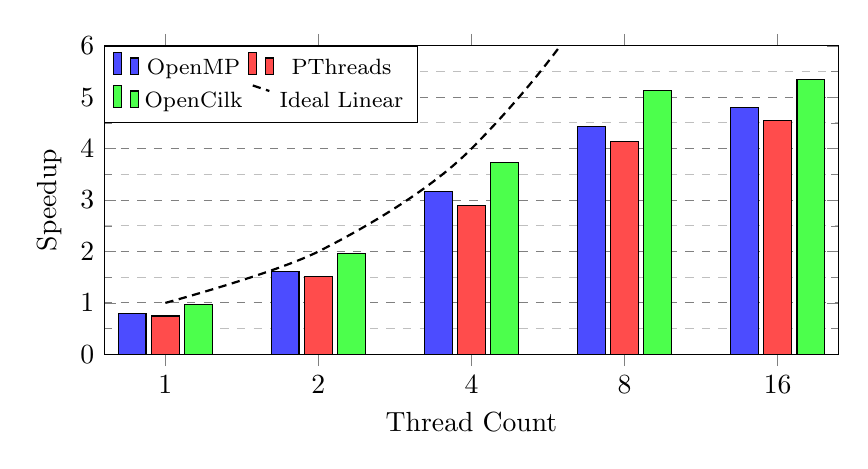
\begin{tikzpicture}
		\begin{axis}[
			ybar,
			width=0.9\textwidth,
			height=5.5cm,
			bar width=10pt,
			ylabel={Speedup},
			xlabel={Thread Count},
			symbolic x coords={1, 2, 4, 8, 16},
			xtick=data,
			legend style={at={(0,1)}, anchor=north west, legend columns=2, font=\footnotesize},
			ymin=0,
			ymax=6,
			ymajorgrids=true,
			yminorgrids=true,
			minor y tick num=1,
			grid style={dashed, black!50},
			ytick={0,1,2,3,4,5,6},
			minor grid style={dashed, gray!50},
		]

		% OpenMP
		\addplot[fill=blue!70] coordinates {
			(1,0.8014) (2,1.6167) (4,3.1708) (8,4.4388) (16,4.8034)
		};

		% PThreads
		\addplot[fill=red!70] coordinates {
			(1,0.7446) (2,1.5069) (4,2.9004) (8,4.1318) (16,4.5467)
		};

		% OpenCilk
		\addplot[fill=green!70] coordinates {
			(1,0.9714) (2,1.9574) (4,3.7305) (8,5.1351) (16,5.3512)
		};

		\addplot[black, densely dashed, thick, smooth] coordinates {
			(1,1) (2,2) (4,4) (8,8) (16,16)
		};

		\legend{OpenMP, PThreads, OpenCilk, Ideal Linear}

		\end{axis}
	\end{tikzpicture} \vspace{-12pt}
	\caption{Strong scaling analysis for label propagation on LiveJournal dataset 
	(1-16 threads). Dashed line indicates ideal linear speedup.}
	\label{fig:thread-speedup}
\end{figure}

\section{Analysis and Discussion}

\subsection{Key Findings}

\begin{itemize}
	\item \textbf{Algorithm Behaviour:} Label propagation (V0) consistently achieves higher speedups (3.14×–5.39×)
	compared to union-find (V1), with efficiencies ranging from 39–67\%. Union-find shows better
	absolute performance but lower parallelization benefits due to more complex data dependencies.

	\item \textbf{Implementation Comparison:} OpenCilk demonstrates superior performance for label propagation
	on most datasets, benefiting from its work-stealing scheduler. OpenMP achieves competitive results
	with simpler code. PThreads consistently shows slightly lower performance due to static work
	partitioning.

	\item\textbf{Dataset Characteristics:} Social networks (Orkut, LiveJournal) exhibit excellent speedups (5.11×–
	5.39×) due to well-balanced component structures. Large sparse graphs (MAWI, Kmer) show modest
	speedups (1.89×–3.14×), likely due to memory bandwidth limitations and irregular access patterns
	that reduce parallel efficiency.

\end{itemize}

\subsection{Notable Observations}
The Hollywood dataset exhibits surprising OpenCilk union-find slowdown (0.81×), 
likely from excessive work-stealing overhead on irregular edge distributions. 
Efficiency metrics reveal none exceed 68\%, indicating memory bandwidth, rather 
than computation, becomes the bottleneck—consistent with the sub-linear scaling 
in Figure \ref{fig:thread-speedup}, where speedup plateaus beyond 4 threads.

\subsection{Strong Scaling Analysis}
Figure \ref{fig:thread-speedup} demonstrates strong scaling behavior for label propagation on 
LiveJournal. All implementations achieve near-linear speedup up to 4 threads 
(OpenCilk: 3.6×, OpenMP: 3.4×), but show diminishing returns at 8 threads 
(OpenCilk: 5.1×, efficiency 64\%) and saturation at 16 threads. This plateau 
reflects Amdahl's Law limitations and memory bandwidth saturation. The gap 
between actual and ideal linear speedup (dashed line) quantifies parallelization 
overhead, with OpenCilk's work-stealing providing 15-20\% advantage over static 
partitioning at higher thread counts.

\subsection{Correctness Verification}
All implementations were verified by comparing component counts across sequential and parallel
versions. Identical results across all implementations confirm correctness, with deterministic
outcomes being the main goal, despite non-deterministic thread scheduling.

\section{Conclusions}
This project successfully demonstrates parallel connected components detection across diverse graph
datasets using multiple programming paradigms. OpenCilk with label propagation achieves the best
results on social network graphs (up to 5.39× speedup with 67\% efficiency), while showing that
memory-bound operations limit scalability on larger sparse graphs. The implemented optimizations—
work chunking, pointer jumping, bitmap-based counting, and thread-local variables—prove essential
for achieving good parallel performance.

\subsection{Future Directions}
Several promising directions for future work include:
\begin{itemize}
	\item Exploring distributed-memory implementations using MPI for graphs exceeding single-node
	capacity
	\item Investigating GPU acceleration using CUDA or OpenCL for massive parallelism
	\item Implementing hybrid algorithms that adaptively switch between label propagation and union-find
	based on graph characteristics
	\item Optimizing memory access patterns through graph reordering and compression techniques
	\item Conducting deeper analysis of cache performance using hardware counters (cache misses,
	memory bandwidth utilization)
\end{itemize}

\textbf{Code Availability:} Complete source code, build instructions, and benchmark scripts are available at
\url{https://github.com/gianst2004/pardis2025}

\end{document}
